% https://tex.stackexchange.com/questions/144826/how-do-i-create-a-tikz-mindmap-that-has-two-connected-roots
\documentclass[landscape]{standalone}
\usepackage{tikz}
\usetikzlibrary{mindmap}

\pagestyle{empty}
\begin{document}

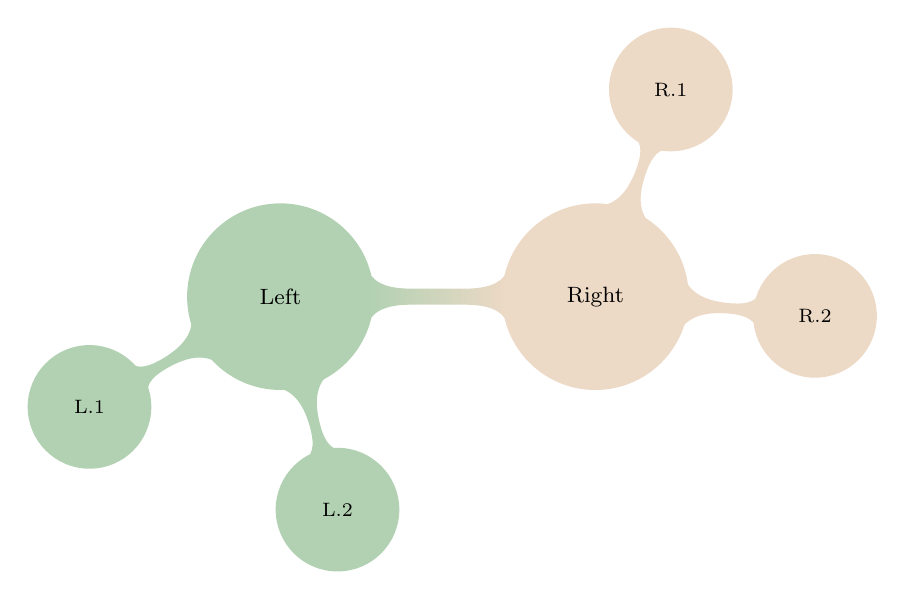
\begin{tikzpicture}[small mindmap, outer sep=0pt, text=black]

  \begin{scope}[concept color=brown!30]
    \node (right) at (2,0) [concept] {Right}
      [clockwise from=70]
      child { node[concept] {R.1} }
      child { node[concept] {R.2} }
    ;
  \end{scope}

  \begin{scope}[concept color=green!40!black!30]
    \node (left) at (-2,0) [concept] {Left}
      [counterclockwise from=210]
      child { node[concept] {L.1}  }
      child { node[concept] {L.2} }
    ;
  \end{scope}
  \path (left) to[circle connection bar switch color=from (green!40!black!30) to (brown!30)] (right) ;

\end{tikzpicture}
\end{document}